% Claim-specific evidence profile. Categories are complementary, not ordinal scores.
\definecolor{profileNavy}{HTML}{183747}
\definecolor{profileTeal}{HTML}{247B80}
\definecolor{profileGold}{HTML}{B68A36}
\definecolor{profileLine}{HTML}{CBD6DB}
\definecolor{profilePale}{HTML}{F3F7F8}
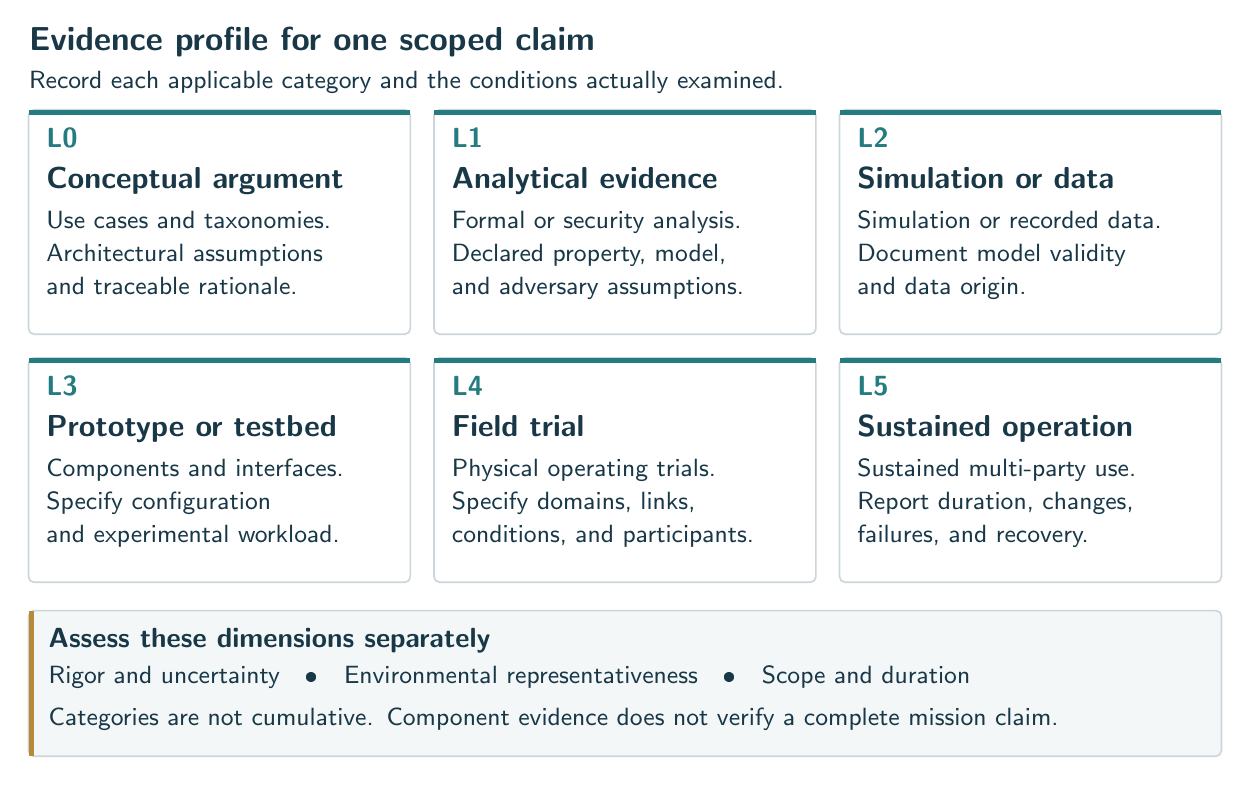
\begin{tikzpicture}[font=\sffamily,text=profileNavy]
  \node[anchor=north west,inner sep=0pt,font=\sffamily\bfseries\fontsize{13}{16}\selectfont]
    at (0,1.05) {Evidence profile for one scoped claim};
  \node[anchor=north west,inner sep=0pt,font=\sffamily\fontsize{9.5}{12}\selectfont]
    at (0,0.50) {Record each applicable category and the conditions actually examined.};

  \foreach \x/\y/\code/\heading/\body in {
    0/0/L0/Conceptual argument/{Use cases and taxonomies.\\Architectural assumptions\\and traceable rationale.},
    5.15/0/L1/Analytical evidence/{Formal or security analysis.\\Declared property, model,\\and adversary assumptions.},
    10.30/0/L2/Simulation or data/{Simulation or recorded data.\\Document model validity\\and data origin.},
    0/-3.15/L3/Prototype or testbed/{Components and interfaces.\\Specify configuration\\and experimental workload.},
    5.15/-3.15/L4/Field trial/{Physical operating trials.\\Specify domains, links,\\conditions, and participants.},
    10.30/-3.15/L5/Sustained operation/{Sustained multi-party use.\\Report duration, changes,\\failures, and recovery.}
  }{
    \path[draw=profileLine,fill=white,line width=0.6pt,rounded corners=2pt]
      (\x,\y) rectangle ++(4.85,-2.85);
    \path[fill=profileTeal] (\x,\y) rectangle ++(4.85,-0.06);
    \node[anchor=north west,inner sep=0pt,font=\sffamily\bfseries\fontsize{10}{12}\selectfont,text=profileTeal]
      at (\x+0.22,\y-0.23) {\code};
    \node[anchor=north west,inner sep=0pt,text width=4.35cm,
      font=\sffamily\bfseries\fontsize{10.5}{13}\selectfont]
      at (\x+0.22,\y-0.72) {\heading};
    \node[anchor=north west,inner sep=0pt,text width=4.35cm,align=left,
      font=\sffamily\fontsize{9.5}{12}\selectfont]
      at (\x+0.22,\y-1.28) {\body};
  }

  \path[draw=profileLine,fill=profilePale,line width=0.6pt,rounded corners=2pt]
    (0,-6.36) rectangle (15.15,-8.21);
  \path[fill=profileGold] (0,-6.36) rectangle (0.065,-8.21);
  \node[anchor=north west,inner sep=0pt,font=\sffamily\bfseries\fontsize{10}{12}\selectfont]
    at (0.25,-6.58) {Assess these dimensions separately};
  \node[anchor=north west,inner sep=0pt,text width=14.55cm,align=left,
    font=\sffamily\fontsize{9.5}{12}\selectfont]
    at (0.25,-7.06) {Rigor and uncertainty\quad\textbullet\quad Environmental representativeness\quad\textbullet\quad Scope and duration\\[3pt]
    Categories are not cumulative. Component evidence does not verify a complete mission claim.};
\end{tikzpicture}
